% !TeX root = ../build/main.tex

This chapter provides an overview of the operational workflow of the Vocdoni Z protocol, detailing the sequential phases and roles involved. The process includes the initialization of a voting event, distributed key generation, encrypted vote casting, vote verification, and accumulation, culminating in the publication and public verification of results. Each phase leverages advanced cryptographic techniques to ensure the integrity, privacy, and universal verifiability of the voting process.

\subsection{Simplified Workflow Steps}

\begin{enumerate}
	\item \textbf{Organizer Creates a New Voting Process}
	
		\begin{itemize}
			\item Prepare the census data.
			\item Set voting details such as duration, options, type, etc.
			\item Send the transaction to the Ethereum Process smart contract.
		\end{itemize}
	
	\item \textbf{Sequencers Create the Distributed Threshold Encryption Key}
	
			\begin{itemize}
				\item Use the Sequencer Registry smart contract to coordinate the Distributed Key Generation (DKG).
				\item Provide collateral to ensure correct participation in the DKG.
				\item Download all required data to handle the new vote, such as the census Merkle tree.
			\end{itemize}
	
	\item \textbf{Voting Begins Once the Encryption Public Key (EPK) is Available}
	
	\item \textbf{Voters Cast Their Votes}

			\begin{itemize}
				\item Choose any of the available sequencers.
				\item Fetch their census Merkle proof to prove eligibility.
				\item Use the EPK to encrypt their voting choice.
				\item Generate a zkSNARK to prove the validity of the encrypted vote and adherence to ballot protocol rules.
				\item Send the encrypted vote, Merkle proof, validify proof and identity proof to the sequencer.
			\end{itemize}
	 
	\item \textbf{Sequencers Verify and Accumulate the Votes}

			\begin{itemize}
				\item Fetch Current State: Retrieve the current valid process state root from the Ethereum smart contract and the associated data from Ethereum blobs.
				\item Generate a zkSNARK of state transition, proving: 
						\begin{itemize}
							\item the validity of the zkSNARK proof provided by the voter.
							\item the correct accumulation of votes from users, adding them to the process state.
							\item the correct sum off the new encrypted votes using the homomorphic properties of ElGamal.
							\item the new votes are from eligible users by checking the census Merkle proofs.
							\item the new voters have not already voted by checking their nullifiers, or it is a correct vote overwrite
							\item the data blob hash matches the data used to verify the transition.
						\end{itemize}
				\item Submit Updated State: Send the new state root to the smart contract and store the updated data in Ethereum blobs.
			\end{itemize}
	
	\item \textbf{Smart Contract Verification of the State Transition}

			\begin{itemize}
				\item Verify the zkSNARK proof provided by the sequencer.
				\item Ensure the origin root corresponds to the current stored state root.
				\item Confirm that the blob hash matches the one stored in Ethereum.
			\end{itemize}
	
	\item \textbf{Repeat Until Voting Ends}

			\begin{itemize}
				\item Sequencers accumulate more votes and create state transitions until the finalization of the process.
			\end{itemize}
	
	\item \textbf{Create the Decryption Key}

			\begin{itemize}
				\item Once voting is complete, sequencers publish their shares of the EPK to the Ethereum smart contract.
				\item Decrypt Results: When the threshold of shares is reached, the results can be decrypted by anyone.
				\item Sequencers receive reward for their correct participation depending on the number of sequenced votes.
			\end{itemize}
	
	\item \textbf{Public Verification of the Final Results}
			\begin{itemize}
				\item After the voting period ends and the results are decrypted, anyone can verify the correctness of the final result.
				\item Use the zkSNARK State proof and publicly available data on-chain to ensure the integrity and correctness of the entire voting process.
			\end{itemize} 
\end{enumerate}

\begin{figure}[H]
	\centering
	\fbox{
		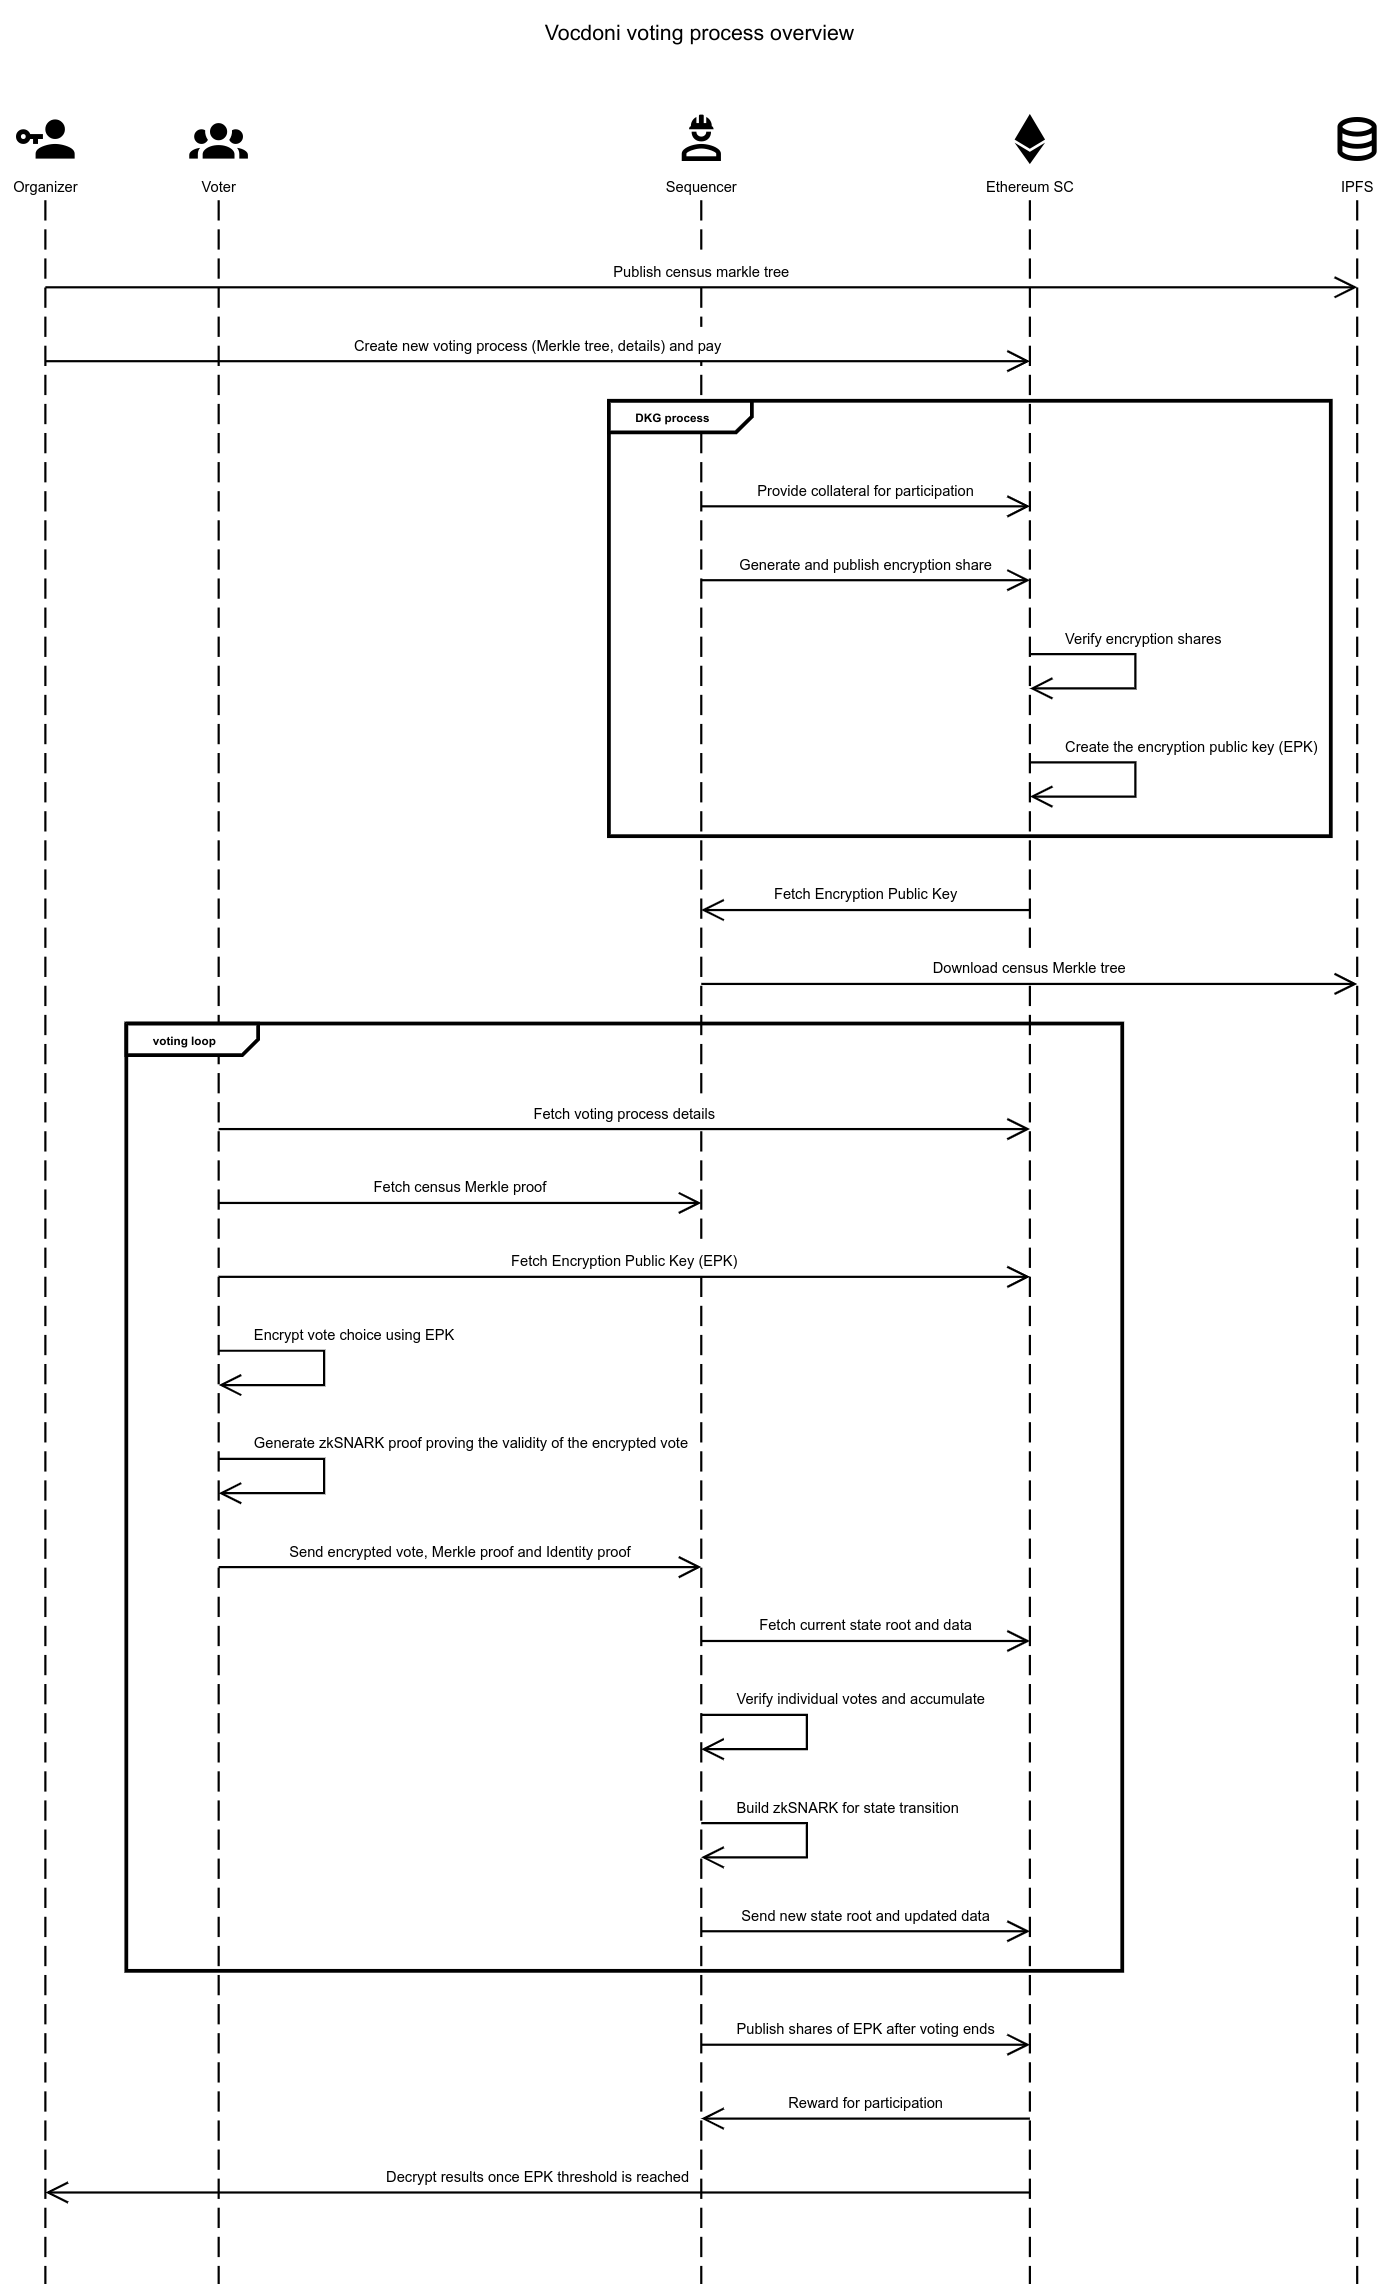
\includegraphics[scale = 0.3, draft = false]{\figs/workflow-simplified.png}}
\end{figure}
